\documentclass[onecolumn]{report}
\usepackage[utf8]{inputenc}
\usepackage{graphicx}
\usepackage{hyperref}
\usepackage{geometry}
\usepackage{times}
\usepackage{float}
\usepackage{multirow}
\usepackage{multicol}
\usepackage{amsmath}
\usepackage{tikz}
\usepackage{subfigure}
\geometry{a4paper,scale=0.8}
\usepackage{algorithm}
\usepackage{algpseudocode}
\usepackage{listings}
\usepackage{booktabs}
\usepackage{url}
\usepackage[hyphenbreaks]{breakurl}
\def\UrlBreaks{\do\A\do\B\do\C\do\D\do\E\do\F\do\G\do\H\do\I\do\J
\do\K\do\L\do\M\do\N\do\O\do\P\do\Q\do\R\do\S\do\T\do\U\do\V
\do\W\do\X\do\Y\do\Z\do\[\do\\\do\]\do\^\do\_\do\`\do\a\do\b
\do\c\do\d\do\e\do\f\do\g\do\h\do\i\do\j\do\k\do\l\do\m\do\n
\do\o\do\p\do\q\do\r\do\s\do\t\do\u\do\v\do\w\do\x\do\y\do\z
\do\.\do\@\do\\\do\/\do\!\do\_\do\|\do\;\do\>\do\]\do\)\do\,
\do\?\do\'\do+\do\=\do\#}



\begin{document}
\title{Summary of COMP523 Advanced Algorithm}
\maketitle
\chapter{Symmetry Notation}
\section{Asymptotic Notation}
Asymptotic notation is a way of describing the limiting behavior of a function when the argument tends towards a particular value or infinity. In computer science, asymptotic notation is frequently used to describe the running time or space usage of an algorithm.\\
\begin{itemize}
\item $O$-notation: $f(n) = O(g(n))$ if there exist constants $c$ and $n_0$ such that $0 \leq f(n) \leq cg(n)$ for all $n \geq n_0$.
\item $\Omega$-notation: $f(n) = \Omega(g(n))$ if there exist constants $c$ and $n_0$ such that $0 \leq cg(n) \leq f(n)$ for all $n \geq n_0$.
\item $\Theta$-notation: $f(n) = \Theta(g(n))$ if there exist constants $c_1$, $c_2$ and $n_0$ such that $0 \leq c_1g(n) \leq f(n) \leq c_2g(n)$ for all $n \geq n_0$.
\item $o$-notation: $f(n) = o(g(n))$ if for any constant $c > 0$, there exists a constant $n_0$ such that $0 \leq f(n) < cg(n)$ for all $n \geq n_0$.
\item $\omega$-notation: $f(n) = \omega(g(n))$ if for any constant $c > 0$, there exists a constant $n_0$ such that $0 \leq cg(n) < f(n)$ for all $n \geq n_0$.
\end{itemize}

\section{Comparing Functions}
\subsection{Transitivity}
\begin{itemize}
\item $f(n) = O(g(n))$ and $g(n) = O(h(n))$ implies $f(n) = O(h(n))$.
\item $f(n) = \Omega(g(n))$ and $g(n) = \Omega(h(n))$ implies $f(n) = \Omega(h(n))$.
\item $f(n) = \Theta(g(n))$ and $g(n) = \Theta(h(n))$ implies $f(n) = \Theta(h(n))$.
\end{itemize}
For example, $n^2 = O(n^3)$ and $n^3 = O(n^4)$ implies $n^2 = O(n^4)$.

\subsection{Reflexivity}
\begin{itemize}
\item $f(n) = O(f(n))$.
\item $f(n) = \Omega(f(n))$.
\item $f(n) = \Theta(f(n))$.
\end{itemize}
For example, $n^2 = O(n^2)$.

\subsection{Symmetry}
\begin{itemize}
\item $f(n) = O(g(n))$ implies $g(n) = O(f(n))$.
\item $f(n) = \Omega(g(n))$ implies $g(n) = \Omega(f(n))$.
\item $f(n) = \Theta(g(n))$ implies $g(n) = \Theta(f(n))$.
\item $f(n) = o(g(n))$ implies $g(n) = \omega(f(n))$.
\item $f(n) = \omega(g(n))$ implies $g(n) = o(f(n))$.
\end{itemize}
For example, $n^2 = O(n^3)$ implies $n^3 = \Omega(n^2)$.

\subsection{Transpose Symmetry}
\begin{itemize}
\item $f(n) = O(g(n))$ if and only if $g(n) = \Omega(f(n))$.
\item $f(n) = \Theta(g(n))$ if and only if $g(n) = \Theta(f(n))$.
\item $f(n) = o(g(n))$ if and only if $g(n) = \omega(f(n))$.
\item $f(n) = \omega(g(n))$ if and only if $g(n) = o(f(n))$.
\end{itemize}
For example, $n^2 = O(n^3)$ if and only if $n^3 = \Omega(n^2)$.\\

\subsection{sum and maximum}
\begin{equation*}
    f_1(n) + f_2(n)+\dots +f_k(n) = \Theta(\max(f_1(n), f_2(n), \dots, f_k(n)))
\end{equation*}
where $k$ is a constant positive integer.\\
Let $f_j(n) = j$, $k=n$, then
\begin{equation*}
    f_1(n) + f_2(n)+\dots +f_k(n) = n(n+1)/2 = \Theta(n^2)
\end{equation*}

\subsection{Running time hierarchy}
\begin{itemize}
    \item logarithmic: $O(\log n)$
    \item linear: $O(n)$
    \item $n\log n$: $O(n\log n)$
    \item quadratic: $O(n^2)$
    \item polynomial: $O(n^k)$
    \item exponential: $O(c^n)$
    \item constant: $O(1)$
    \item superconstant: $\omega (1)$
    \item sublinear: $o(n)$
    \item superlinear: $\omega (n)$
    \item superpolynomial: $\omega (n^k)$
    \item subexponential: $o(c^n)$
\end{itemize}

\section{Expect of algorithms}
\textbf{Correctness}: An algorithm is correct if it halts with the correct output for every input instance.\\
\textbf{Termination}: An algorithm is terminating if it halts for every input instance.\\
\textbf{Efficiency}: An algorithm is efficient if it halts with the correct output for every input instance and runs in polynomial time.\\

\chapter{Recursion and Divide and Conquer techniques}
\section{Finding Majority in array}
The pesudocode of the algorithm is shown in Algorithm \ref{alg:majority}.
\begin{algorithm}
\label{alg:majority}
\caption{Finding Majority in array}
\begin{algorithmic}[1]
\Procedure{Majority}{$A$}
\State $n \gets \text{length of } A$
\If {$n = 0$}
\State \textbf{return} $-1$
\EndIf
\If {$n = 1$}
\State \textbf{return} $A[1]$
\EndIf
\If {$n \large 1$ and $n$ is odd}
\State 
\EndIf
\State Array $B$ of size $n/2$
\State set $j$=0
\For {$i=1$ to $n/2$}
\If {$A[2i-1] = A[2i]$}
\State $B[j] \gets A[2i-1]$
\State $j \gets j+1$
\EndIf
\EndFor
\State $m \gets \textsc{Majority}(B)$
\State $count \gets 0$
\For {$i=1$ to $n$}
\If {$A[i] = m$}
\State $count \gets count+1$
\EndIf
\EndFor
\If {$count > n/2$}
\State \textbf{return} $m$
\Else
\State \textbf{return} $-1$
\EndIf
\EndProcedure
\end{algorithmic}
\end{algorithm}\\
\textbf{Correctness}:\\
Lemma: If $A$ has a majority element, then the majority element of $A$ is also the majority element of $B$.\\
Base case: $n=1$, the majority element is $A[1]$.\\
Induction hypothesis: Assume that the lemma is true for $n=k$, we will prove that the lemma is true for $n=k+1$.\\
Induction step: If $A$ has a majority element, then the majority element of $A$ is also the majority element of $B$.\\
Case 1 ($A$ has a majority element $m$): Then by the lemma, it is also the majority element of $B$. Then $m$ appears more than $k/2$ times in $B$. Then $m$ appears more than $(k+1)/2$ times in $A$.\\
Case 2 ($A$ has no majority element): Then $B$ has no majority element. Then $A$ has no majority element.\\
\textbf{Proof the lemma}:\\
proof by contradiction. Assume that $A$ has a majority element $m$ and $B$ has a majority element $m'$, but $m \neq m'$. \\
Let $x$ be the numbers of occurrence of $m$ in $A$.\\
Let $y$ be the numbers of occurrence of $m'$ in $B$.\\
Then $2y$ times from pairs that are represented in $B$ by a value different from $m'$, and $x-2y$ times, since each occurrence of $m$ in $A$ that is not paired with another occurrence of $m$ in $A$ is paired with an occurrence of $m'$ in $B$.\\
In total, this gives $2y+x-2y=x$ occurrences of $m$ in $A$, which is a contradiction.\\
\textbf{Running time}:\\
Recursive formula for the running time:
\begin{equation*}
    T(n) \leq T(n/2) + cn
\end{equation*}
where $c$ is a constant.\\
The solution to the recurrence is $T(n) = O(n)$.\\

\section{Searching in logarithmic time}
Searching faster with BinarySearch.\\
It is a particular case of the divide-and-conquer paradigm.\\
\textbf{Input}: A sorted array $A$ of $n$ elements and a value $x$.\\
\textbf{Output}: An index $i$ such that $A[i] = x$ or the special value $-1$ if $x$ does not appear in $A$.\\
\textbf{Pseudocode} is shown in Algorithm \ref{alg:binarysearch}.
\begin{algorithm}
\label{alg:binarysearch}
\caption{BinarySearch}
\begin{algorithmic}[1]
\Procedure{BinarySearch}{$x,i,j$}
\If {$i=j$}
\If {$A[i] = x$}
\State \textbf{return} $i$
\Else
\State \textbf{return} $-1$
\EndIf
\Else
\If {$x=A[\lfloor (i+j)/2 \rfloor]$}
\State \textbf{return} $\lfloor (i+j)/2 \rfloor$
\ElsIf {$x<A[\lfloor (i+j)/2 \rfloor]$}
\State \textbf{return} $\textsc{BinarySearch}(x,i,\lfloor (i+j)/2 \rfloor)$
\Else
\State \textbf{return} $\textsc{BinarySearch}(x,\lfloor (i+j)/2 \rfloor+1,j)$
\EndIf
\EndIf
\EndProcedure
\end{algorithmic}
\end{algorithm}\\
\textbf{Running time}:\\
The number of comparisons performed by BinarySearch is:\\
\begin{equation*}
    T(n) \leq  T(n/2) + 4  
\end{equation*}
Keep calculate:
\begin{align*}
    T(n) &\leq T(n/2) + 4\\
    &\leq T(n/4) + 4 + 4\\
    &\leq T(n/8) + 4 + 4 + 4\\
    &\leq T(n/2^k) + 4k\\
    &\leq T(n/2^{\log (n-1)}) + 4\log (n-1)\\
    &= T(2) + 4(\log n-1)\\
    &\leq 4\log n - 4\\
    &= 4\log n\\
\end{align*}
proof $T(n) \leq 4\log n$:\\
Base case: $n=1$, $T(1) = 0 \leq 4\log 1 = 0$.\\
Induction hypothesis: Assume that the lemma is true for $n=k$, we will prove that the lemma is true for $n=k+1$.\\
Induction step: $T(k+1) \leq 4\log (k+1)$.\\
\begin{align*}
    T(k+1) &\leq T(k/2) + 4\\
    &\leq 4\log (k/2) + 4\\
    &= 4\log k - 4 + 4\\
    &= 4\log k\\
    &\leq 4\log (k+1)
\end{align*}
\textbf{Memory usage}:\\
The memory usage of BinarySearch is:\\
\begin{equation*}
    M(n) = O(\log n)
\end{equation*}
\textbf{Comparing BinarySearch and LinearSearch}:\\
\begin{equation*}
    T_{\text{BinarySearch}}(n) = O(\log n)
\end{equation*}
\begin{equation*}
    T_{\text{LinearSearch}}(n) = O(n)
\end{equation*}
\begin{equation*}
    T_{\text{BinarySearch}}(n) = O(\log n) < O(n) = T_{\text{LinearSearch}}(n)  
\end{equation*}
\begin{equation*}
    M_{\text{BinarySearch}}(n) = O(\log n) < O(1) = M_{\text{LinearSearch}}(n)
\end{equation*}

\section{Running time of Divide and Conquer algorithms}
The Master Theorem:\\
Suppose that $T(n)$ satisfies the recurrence:
\begin{equation*}
    T(n) \leq aT(n/b) + cn^d
\end{equation*}
where $a \geq 1$, $b > 1$, $c > 0$ and $d \geq 0$ are constants.\\
Then $T(n)$ has the following asymptotic bounds:\\
\begin{equation*}
    T(n) = \begin{cases}
    O(n^d) & \text{if } d > \log_b a\\
    O(n^d\log n) & \text{if } d = \log_b a\\
    O(n^{\log_b a}) & \text{if } d < \log_b a
    \end{cases}
\end{equation*}
This theorem is useful for solving recurrences of the form:
\begin{equation*}
    T(n) = aT(n/b) + f(n)
\end{equation*}
where $a \geq 1$, $b > 1$ and $f(n)$ is an asymptotically positive function.\\
\textbf{Example}:\\
\begin{equation*}
    T(n) = 8T(n/2) + 100n^2
\end{equation*}
$a = 8$, $b = 2$, $f(n) = 100n^2$, $d = 2$, $\log_b a = \log_2 8 = 3$.\\
$d = 2 < \log_b a = 3$, so $T(n) = O(n^{\log_b a}) = O(n^3)$.\\

\section{Finding piar of points closest to each other}
\textbf{Input}: A set $P$ of $n$ points in the plane.\\
\textbf{Output}: The pair of points in $P$ that are closest to each other.\\
\textbf{Pseudocode} is shown in Algorithm \ref{alg:closestpair}.
\begin{algorithm}
\label{alg:closestpair}
\caption{ClosestPair}
\begin{algorithmic}[1]
\Procedure{ClosestPair}{$P_1,\dots,P_n$}
\State Construct $P_x$ and $P_y$. $P_x$ is sorted by $x$-coordinate, $P_y$ is sorted by $y$-coordinate.
\State \textbf{return} $\textsc{ClosestPairRec}(P_x,P_y)$
\EndProcedure
\end{algorithmic}
\end{algorithm}
\begin{algorithm}
\caption{ClosestPairRec}
\begin{algorithmic}[1]
\Procedure{ClosestPairRec}{$P_x,P_y$}
\If {$|P_x|=|P_y| \leq 3$}
\State For each pair of points $(P_i,P_j)$, compute $d(P_i,P_j)$
\State \textbf{return} the pair of points with the smallest distance
\EndIf
\State Construct $Q_x$, $Q_y$, $R_x$ and $R_y$.
\State ($l_1,l_2$) = \textsc{ClosestPairRec}($Q_x,Q_y$)
\State ($r_1,r_2$) = \textsc{ClosestPairRec}($R_x,R_y$)
\State $\delta = \min\{d(l_1,l_2),d(r_1,r_2)\}$
\State $x^*$ = the largest $x$-coordinate in $Q_x$
\State $L = {(x,y):x=x^*}$
\State $S = \{p \in P: p \in L \text{ and } p \text{ is within } \delta \text{ of } L\}$
\State Construct $S_v$ 
\For {$p \in S$}
\State Let $q$ be the point in $S_v$ closest to $p$
\If {$d(p,q) < \delta$}
\State $\delta = d(p,q)$
\State ($s_1,s_2$) = ($p,q$)
\EndIf
\EndFor
\If {$d(s_1,s_2) < \min\{d(l_1,l_2),d(r_1,r_2)\}$}
\State \textbf{return} ($s_1,s_2$)
\EndIf
\If {$d(l_1,l_2) < d(r_1,r_2)$}
\State \textbf{return} ($l_1,l_2$)
\Else
\State \textbf{return} ($r_1,r_2$)
\EndIf
\EndProcedure
\end{algorithmic}
\end{algorithm}
\textbf{Running time}:\\
$T(n) \leq 2T(n/2) + O(n\log n) = O(n\log n)$\\
\textbf{Example}:\\

\chapter{Graph Algorithms}
\section{Graph Definitions}
\textbf{Graph}: A graph $G$ consists of a set $V$ of vertices and a set $E$ of edges, where each edge is associated with a pair of vertices.\\
\textbf{Directed Graph}: A directed graph $G$ consists of a set $V$ of vertices and a set $E$ of directed edges, where each directed edge is associated with an ordered pair of vertices.\\
\textbf{Undirected Graph}: An undirected graph $G$ consists of a set $V$ of vertices and a set $E$ of undirected edges, where each undirected edge is associated with an unordered pair of vertices.\\
\textbf{Neighbours of a vertex $v$}: Set of vertices that are connected to $v$ by an edge.\\
\textbf{Degree of a vertex $v$}: number of neighbours of $v$, denoted by $deg(v)$.\\
\textbf{Path}: A sequence of (non-repeating) nodes with consecutive nodes being connected by an edge.\\
length = node count - 1 = edge count.\\
\textbf{Distance between two nodes}: The number of edges in the shortest path between the two nodes.\\
\textbf{Graph diameter}: The maximum distance between any two nodes in the graph.\\

\textbf{Lines,cycles,trees and cliques}:\\
\textbf{Line}: A graph with $n$ vertices and $n-1$ edges.\\
\textbf{Cycle}: A graph with $n$ vertices and $n$ edges.\\
\textbf{cliques}: A graph with $n$ vertices and $n(n-1)/2$ edges.\\
\textbf{Tree}: A graph with $n$ vertices and $n-1$ edges.\\

\textbf{Graph representations}:\\
\textbf{Adjacency matrix}: A $n \times n$ matrix $A$ where $A_{ij} = 1$ if there is an edge between $i$ and $j$, and $A_{ij} = 0$ otherwise.\\
examples of adjacency matrices:\\
Given the following graph:\\
\begin{center}
    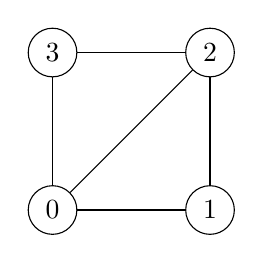
\begin{tikzpicture}
\node[shape=circle,draw=black] (A) at (0,0) {0};
\node[shape=circle,draw=black] (B) at (2,0) {1};
\node[shape=circle,draw=black] (C) at (2,2) {2};
\node[shape=circle,draw=black] (D) at (0,2) {3};
\path [-] (A) edge node[left] {} (B);
\path [-] (B) edge node[left] {} (C);
\path [-] (C) edge node[left] {} (D);
\path [-] (D) edge node[left] {} (A);
\path [-] (A) edge node[left] {} (C);
\end{tikzpicture}\\
\end{center}
The adjacency matrix is:\\
\begin{equation*}
    \begin{bmatrix}
    0 & 1 & 1 & 1\\
    1 & 0 & 1 & 0\\
    1 & 1 & 0 & 1\\
    1 & 0 & 1 & 0
    \end{bmatrix}
\end{equation*}
\textbf{Adjacency matrix for directed graphs}: A $n \times n$ matrix $A$ where $A_{ij} = 1$ if there is an edge from $i$ to $j$, and $A_{ij} = 0$ otherwise.\\
examples of adjacency matrices for directed graphs:\\
Given the following graph:\\
\begin{center}
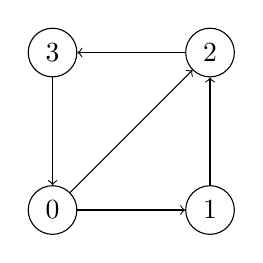
\begin{tikzpicture}
\node[shape=circle,draw=black] (A) at (0,0) {0};
\node[shape=circle,draw=black] (B) at (2,0) {1};
\node[shape=circle,draw=black] (C) at (2,2) {2};
\node[shape=circle,draw=black] (D) at (0,2) {3};
\path [->] (A) edge node[left] {} (B);
\path [->] (B) edge node[left] {} (C);
\path [->] (C) edge node[left] {} (D);
\path [->] (D) edge node[left] {} (A);
\path [->] (A) edge node[left] {} (C);
\end{tikzpicture}\\
\end{center}
The adjacency matrix is:\\
\begin{equation*}
    \begin{bmatrix}
    0 & 1 & 0 & 0\\
    0 & 0 & 1 & 0\\
    0 & 0 & 0 & 1\\
    1 & 0 & 0 & 0
    \end{bmatrix}
\end{equation*}
\textbf{Adjacency list}: A list of lists, where the $i$th list contains the neighbours of vertex $i$.\\
Given the following graph:\\
\begin{center}
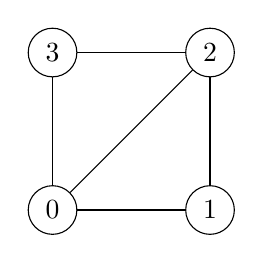
\begin{tikzpicture}
\centering
\node[shape=circle,draw=black] (A) at (0,0) {0};
\node[shape=circle,draw=black] (B) at (2,0) {1};
\node[shape=circle,draw=black] (C) at (2,2) {2};
\node[shape=circle,draw=black] (D) at (0,2) {3};
\path [-] (A) edge node[left] {} (B);
\path [-] (B) edge node[left] {} (C);
\path [-] (C) edge node[left] {} (D);
\path [-] (D) edge node[left] {} (A);
\path [-] (A) edge node[left] {} (C);
\end{tikzpicture}\\
\end{center}
The adjacency list is:\\
\begin{equation*}
    \begin{bmatrix}
    1 & 2 & 3\\
    0 & 2\\
    0 & 1 & 3\\
    0 & 2
    \end{bmatrix}
\end{equation*}
\textbf{Adjacency list for directed graphs}: A list of lists, where the $i$th list contains the neighbours of vertex $i$.\\
Given the following graph:\\
\begin{center}
    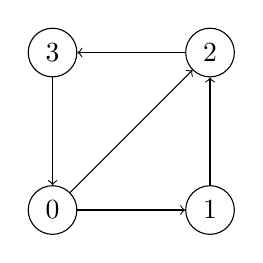
\begin{tikzpicture}
\centering
\node[shape=circle,draw=black] (A) at (0,0) {0};
\node[shape=circle,draw=black] (B) at (2,0) {1};
\node[shape=circle,draw=black] (C) at (2,2) {2};
\node[shape=circle,draw=black] (D) at (0,2) {3};
\path [->] (A) edge node[left] {} (B);
\path [->] (B) edge node[left] {} (C);
\path [->] (C) edge node[left] {} (D);
\path [->] (D) edge node[left] {} (A);
\path [->] (A) edge node[left] {} (C);
\end{tikzpicture}\\
\end{center}

The adjacency list is:\\
\begin{equation*}
    \begin{bmatrix}
    1 & 2\\
    2\\
    3\\
    0
    \end{bmatrix}
\end{equation*}
\textbf{Adjacency matrix vs adjacency list}:\\
\begin{table}[H]
\centering
\begin{tabular}{|c|c|}
\hline
Adjacency matrix & Adjacency list\\
\hline
$O(1)$ to check if there is an edge between $i$ and $j$ & $O(min(deg(i),deg(j)))$ to check if there is an edge between $i$ and $j$\\
\hline
$O(n)$ to find the neighbours of $i$ & $O(deg(j))$ to find the neighbours of $i$\\
\hline
$O(n^2)$ space & $O(n+m)$ space\\
\hline
\end{tabular}
\end{table}

\section{Depth-first search}
\textbf{Depth-first search}: A graph search algorithm that explores the neighbours of a vertex before exploring the neighbours of its neighbours.\\
example of depth-first search:\\
\begin{center}
    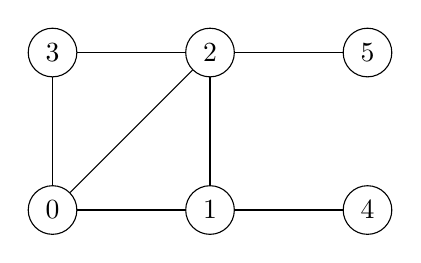
\begin{tikzpicture}
\centering
\node[shape=circle,draw=black] (A) at (0,0) {0};
\node[shape=circle,draw=black] (B) at (2,0) {1};
\node[shape=circle,draw=black] (C) at (2,2) {2};
\node[shape=circle,draw=black] (D) at (0,2) {3};
\node[shape=circle,draw=black] (E) at (4,0) {4};
\node[shape=circle,draw=black] (F) at (4,2) {5};
\path [-] (A) edge node[left] {} (B);
\path [-] (B) edge node[left] {} (C);
\path [-] (C) edge node[left] {} (D);
\path [-] (D) edge node[left] {} (A);
\path [-] (A) edge node[left] {} (C);
\path [-] (E) edge node[left] {} (B);
\path [-] (F) edge node[left] {} (C);
\end{tikzpicture}\\
\end{center}
The depth-first search sequence is:\\
\begin{equation*}
    0,1,2,3,5,4
\end{equation*}
\textbf{Depth-first search algorithm}:\\
\begin{algorithm}[H]
\caption{Depth-first search algorithm}
\begin{algorithmic}[1]
\Procedure{DFS}{$G,v$}
\For {$e \in V$}
\If {$e$ is unexplored}
\State $u$ = head of $e$
\If {$u$ is unexplored}
\State $e$ is a tree edge
\State \Call{DFS}{$G,u$}
\Else
\State $e$ is a back edge
\EndIf
\EndIf
\EndFor
\EndProcedure
\end{algorithmic}
\end{algorithm}
\textbf{Running time of depth-first search}: $O(n+m)$\\


\section{Breadth-first search}
\textbf{Breadth-first search}: A graph search algorithm that explores the neighbours of a vertex before exploring the neighbours of its neighbours.\\
exaqmple of breadth-first search:\\
\begin{center}
    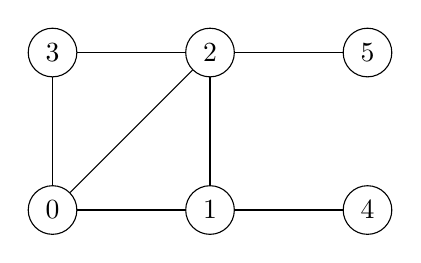
\begin{tikzpicture}
\centering
\node[shape=circle,draw=black] (A) at (0,0) {0};
\node[shape=circle,draw=black] (B) at (2,0) {1};
\node[shape=circle,draw=black] (C) at (2,2) {2};
\node[shape=circle,draw=black] (D) at (0,2) {3};
\node[shape=circle,draw=black] (E) at (4,0) {4};
\node[shape=circle,draw=black] (F) at (4,2) {5};
\path [-] (A) edge node[left] {} (B);
\path [-] (B) edge node[left] {} (C);
\path [-] (C) edge node[left] {} (D);
\path [-] (D) edge node[left] {} (A);
\path [-] (A) edge node[left] {} (C);
\path [-] (E) edge node[left] {} (B);
\path [-] (F) edge node[left] {} (C);
\end{tikzpicture}\\
\end{center}
The breadth-first search sequence starting from vertex 0 is 0, 1, 2, 3, 4, 5.\\
\textbf{Breadth-first search algorithm}:\\
\begin{algorithm}[H]
\caption{Breadth-first search algorithm}
\begin{algorithmic}[1]
\Procedure{BFS}{$G,s$}
\State initial empty list $L$
\State $L \gets {s}$
\State $i \gets 0$
\While{$L[i] \neq \emptyset$}
\State $L_{i+1} \gets empty list$
\For{$v \in L[i]$}
\For{edges $(e)$ incident to $v$}
\If{$e$ is unexplored}
\State $w \gets$ the other end of $e$
\If {$w$ is unexplored}
\State label $e$ as a tree edge
\State add $w$ to $L_{i+1}$
\Else
\State label $e$ as a cross edge
\EndIf
\EndIf
\EndFor
\EndFor
\State $i \gets i+1$
\EndWhile
\EndProcedure
\end{algorithmic}
\end{algorithm}
\textbf{Running time of breadth-first search}: $O(n+m)$\\


\section{Strong Connectivity}
\textbf{Directed graph}: A graph where the edges have a direction.\\
Examples:\\
\begin{center}
    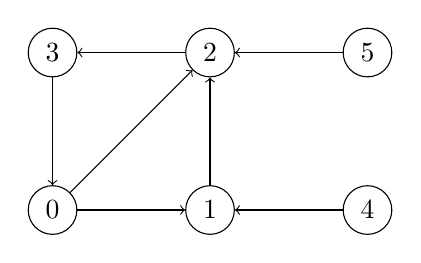
\begin{tikzpicture}
\centering
\node[shape=circle,draw=black] (A) at (0,0) {0};
\node[shape=circle,draw=black] (B) at (2,0) {1};
\node[shape=circle,draw=black] (C) at (2,2) {2};
\node[shape=circle,draw=black] (D) at (0,2) {3};
\node[shape=circle,draw=black] (E) at (4,0) {4};
\node[shape=circle,draw=black] (F) at (4,2) {5};
\path [->] (A) edge node[left] {} (B);
\path [->] (B) edge node[left] {} (C);
\path [->] (C) edge node[left] {} (D);
\path [->] (D) edge node[left] {} (A);
\path [->] (A) edge node[left] {} (C);
\path [->] (E) edge node[left] {} (B);
\path [->] (F) edge node[left] {} (C);
\end{tikzpicture}\\
\end{center}
\noindent
\textbf{DFS and BFS on directed graphs}:\\
Very similar to undirected graphs, except that we only consider edges that go out of a vertex.\\
Running time is $O(n+m)$\\
For example graph above the DFS sequence is 0, 1, 2, 3.\\
The BFS sequence is 0, 1, 2, 3.\\
\subsection{Connectivity}
\textbf{Weak connectivity}:If we ignore the direction for all edges, there would be a pah from any vertex to any other vertex.\\
\textbf{Strong Connectivity}:For every two nodes $u$ and $v$, there is a path from $u$ to $v$ and a path from $v$ to $u$.\\

\subsection{Mutual Reachability}
Two nodes $u$ and $v$ are mutually reachable if there is a path from $u$ to $v$ and a path from $v$ to $u$.\\
\textbf{Strong connectivity}:For every pair of nodes $u$ and $v$, these two nodes are mutually reachable.\\
\textbf{Transitivity}:If $u$ is mutually reachable with $v$ and $v$ is mutually reachable with $w$, then $u$ is mutually reachable with $w$.\\
\\


\subsection{Testing strong connectivity}
\begin{algorithm}[H]
\caption{Testing strong connectivity}
\begin{algorithmic}[1]
\Procedure{TestStrongConnectivity}{$G$}
\State define $G^R$ to be the graph with the same vertices as $G$ but with all edges reversed
\State Select a node $s$ in $G$
\State BFS($G,s$),BFS($G^R,s$)
\For{each node $v$}
\If{$v$ is unexplored in either BFS}
\State \Return False
\EndIf
\EndFor
\State \Return True
\EndProcedure
\end{algorithmic}
\end{algorithm}

\section{Testing bipartiteness}
\textbf{Bipartite graph}: A graph $G=(V,E)$ is bipartite if any only if the vertices can be partitioned into two sets $V_1$ and $V_2$ such that every edge has one end in $V_1$ and the other end in $V_2$.\\
A Graph $G=(V,E)$ is bipartite if and only if it has no odd cycles.(odd cycle: a cycle with odd number of edges)\\
\noindent
\textbf{Testing bipartiteness}:\\
Given a graph $G=(V,E)$, we want to test if $G$ is bipartite.\\
Given a graph $G=(V,E)$, decide if it is 2-colourable.\\
Given a graph $G=(V,E)$, decide if it has an odd cycle.\\
\noindent
\textbf{Colouring the nodes}
It is quite familiar with BFS:\\
\begin{algorithm}[H]
\caption{Colouring the nodes}
\begin{algorithmic}[1]
\Procedure{Colouring}{$G,s$}
\State initial empty list $L$
\State initial empty list $C$
\State $L \gets {s}$
\State $C[s] \gets red$
\State $i \gets 0$
\While{$L[i] \neq \emptyset$}
\State $L_{i+1} \gets empty list$
\For{$v \in L[i]$}
\For{edges $(e)$ incident to $v$}
\If{$e$ is unexplored}
\State $w \gets$ the other end of $e$
\If {$w$ is unexplored}
\State label $e$ as a tree edge
\State add $w$ to $L_{i+1}$
\If {$i+1$ is odd}
\State $C[w] \gets green$
\Else 
\State $C[w] \gets red$
\EndIf
\Else
\State label $e$ as a cross edge
\If{$C[v] = C[w]$}
\State \Return False
\EndIf
\EndIf
\EndIf
\EndFor
\EndFor
\State $i \gets i+1$
\EndWhile
\For {$e(v,w) \in G$}
\If {$C[v] = C[w]$}
\State \Return False
\EndIf
\EndFor
\State \Return True
\EndProcedure
\end{algorithmic}
\end{algorithm}
\noindent
\textbf{Running time of colouring the nodes}: $O(n+m)$\\
\textbf{Correctness of colouring the nodes}:\\
Proof by contradiction.\\
Suppose that $G$ is not bipartite.\\
Then $G$ has an odd cycle.\\
Suppose to the contrary that the algorithm return True.\\
That means that the algorithm did not detect the odd cycle.\\

\section{DAGs and Topological Ordering}
\textbf{DAG}: A directed acyclic graph (DAG) is a directed graph with no directed cycles.\\
examples of DAGs:\\
\begin{center}
    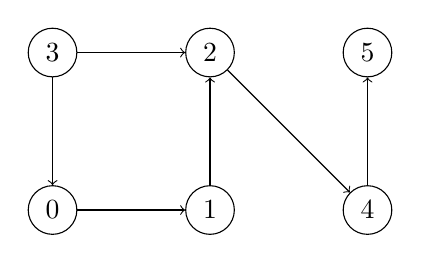
\begin{tikzpicture}
\centering
\node[shape=circle,draw=black] (A) at (0,0) {0};
\node[shape=circle,draw=black] (B) at (2,0) {1};
\node[shape=circle,draw=black] (C) at (2,2) {2};
\node[shape=circle,draw=black] (D) at (0,2) {3};
\node[shape=circle,draw=black] (E) at (4,0) {4};
\node[shape=circle,draw=black] (F) at (4,2) {5};
\path [->] (A) edge node[left] {} (B);
\path [->] (B) edge node[left] {} (C);
\path [->] (C) edge node[left] {} (E);
\path [->] (D) edge node[left] {} (A);
\path [->] (D) edge node[left] {} (C);
\path [->] (E) edge node[left] {} (F);
\end{tikzpicture}\\
\end{center}
\noindent
\textbf{Topological ordering}:Given a graph$G=(V,E)$, a topological ordering of $G$ is an ordering of the nodes $u_1,u_2,\dots,u_n$ such that for every edge $(u_i,u_j)$, we have $i<j$.\\
Intutively, a topological ordering is an ordering of the nodes such that every edge goes from left to right.\\
example of topological ordering based on given graph above:\\
\begin{equation*}
    3,0,1,2,4,5
\end{equation*}
\noindent
\textbf{Topological ordering implies DAG}:\\
\begin{itemize}
    \item If $G$ has a topological ordering, then $G$ is a DAG.
    \item Suppose by contradiction that $G$ has a topological ordering $u_1,u_2,\dots,u_n$ but $G$ also has a cycle $C$.
    \item Let $u_j$ be the smallest element of $C$ in the topological ordering.
    \item Let $u_i$ be its predecessor in $C$.
    \item $u_i$ must appear before $u_j$ in the topological ordering.
    \item This contradicts the fact that $u_j$ is the smallest element of $C$ in the topological ordering.
\end{itemize}

\noindent
\textbf{DAG implies topological ordering}:\\
Proof by induction:
Base case: If $G$ has one or two nodes, then $G$ has a topological ordering.\\
Induction steps: Assume that a DAG up to $k$ nodes has a topological ordering(induction hypothesis). we will prove that a DAG with $k+1$ nodes has a topological ordering.
\begin{itemize}
    \item By our lemma, there is at least one source node in $G$, and let $u$ be the node.
    \item Put $u$ at the beginning of the topological ordering.
    \item Consider the graph $G'$, obtained by $G$ by removing $u$ and its incident edges.
    \item $G'$ is a DAG with $k$ nodes.
    \item It has a topological ordering $u_1,u_2,\dots,u_k$ by the induction hypothesis.
    \item Append this ordering to $u$ to get a topological ordering of $G$.
\end{itemize}
\noindent
Here is the algorithm:\\
\begin{algorithm}[H]
\caption{Topological Sorting}
\begin{algorithmic}[1]
\Procedure{TopologicalSorting}{$G$}
\State find a source vertex $u$
\State set $u$ as the first element of the topological ordering
\State $G' \gets G$ with $u$ and its incident edges removed
\State $L \gets$ \Call{TopologicalSorting}{$G'$}
\State append $L$ to $u$
\EndProcedure
\end{algorithmic}
\end{algorithm}
\noindent
Running time of the algorithm is $O(n^2)$\\
\textbf{Modified Topological Sorting}:\\
Running time of the algorithm is $O(n+m)$\\
\begin{algorithm}[H]
\caption{Modified Topological Sorting}
\begin{algorithmic}[1]
\Procedure{ModifiedTopologicalSorting}{$G$}
\State $L \gets empty list$
\State $S \gets$ set of all source vertices
\While{$S \neq \emptyset$}
\State remove a vertex $u$ from $S$
\State append $u$ to $L$
\For{each edge $(u,v)$}
\State remove edge $(u,v)$ from $G$
\If{$v$ is a source vertex}
\State add $v$ to $S$
\EndIf
\EndFor
\EndWhile
\If{$G$ has edges}
\State \Return $G$ has a cycle
\Else
\State \Return $L$
\EndIf
\EndProcedure
\end{algorithmic}
\end{algorithm}

\section{Finding strongly connected components}
\textbf{connected components}: A connected component of an undirected graph is subgraph of the graph where any two nodes are connected by a path.\\
\textbf{strongly connected components}: A strongly connected component of a directed graph is a subgraph of the graph where any two nodes are mutually reachable.(mutually reachable: there is a path from $u$ to $v$ and a path from $v$ to $u$)\\
\textbf{Finding strongly connected components}:\\
\textbf{Kosaraju's algorithm}:\\
\begin{algorithm}[H]
\caption{Kosaraju's algorithm}
\begin{algorithmic}[1]
\Procedure{Kosaraju}{$G$}
\State Initialise stack $S$
\State Select a arbitrary node $s$
\State DFS\_tree=DFS($G,s$)
\State $S \gets$ nodes in DFS\_tree
\State $G^R \gets$ nodes in order of $S$
\State DFS($G^R,s$)
\State \Return the nodes in the DFS tree
\EndProcedure
\end{algorithmic}
\end{algorithm}
\noindent
\textbf{Running time of Kosaraju's algorithm}: $O(n+m)$\\
\textbf{Correctness of Kosaraju's algorithm}:
\begin{itemize}
    \item Define a meta-graph of $G$, called $G^{SCC}=(V^{SCC},E^{SCC})$.
    \item Supposed that $G$ has strongly connected components (SCCs) $C_1,C_2,\dots,C_k$, for some $k$.
    \item $V^{SCC} = \{C_1,C_2,\dots,C_k\}$ contains some of the SCCs of $G$.
    \item There is an edge $(C_i,C_j)$ in $E^{SCC}$ if $G$ contains a directed edge ($x,y$) such that $x \in C_i$ and $y \in C_j$, crossing different components.
\end{itemize}
\noindent
Examples:
\begin{center}
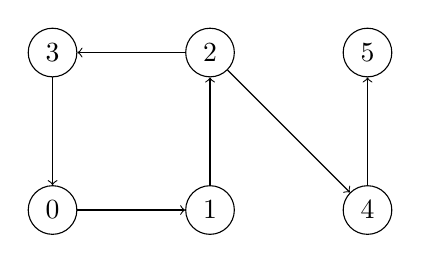
\begin{tikzpicture}
\centering
\node[shape=circle,draw=black] (A) at (0,0) {0};
\node[shape=circle,draw=black] (B) at (2,0) {1};
\node[shape=circle,draw=black] (C) at (2,2) {2};
\node[shape=circle,draw=black] (D) at (0,2) {3};
\node[shape=circle,draw=black] (E) at (4,0) {4};
\node[shape=circle,draw=black] (F) at (4,2) {5};
\path [->] (A) edge node[left] {} (B);
\path [->] (B) edge node[left] {} (C);
\path [->] (C) edge node[left] {} (E);
\path [->] (D) edge node[left] {} (A);
\path [->] (C) edge node[left] {} (D);
\path [->] (E) edge node[left] {} (F);
\end{tikzpicture}\\
\end{center}
\noindent
The SCCs are $\{0,1,2,3\}$ and $\{4,5\}$.\\
\noindent
The meta-graph is:\\
\begin{center}
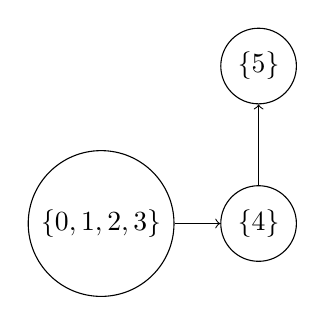
\begin{tikzpicture}
\centering
\node[shape=circle,draw=black] (A) at (0,0) {$\{0,1,2,3\}$};
\node[shape=circle,draw=black] (B) at (2,0) {$\{4\}$};
\node[shape=circle,draw=black] (C) at (2,2) {$\{5\}$};
\path [->] (A) edge node[left] {} (B);
\path [->] (B) edge node[left] {} (C);
\end{tikzpicture}\\
\end{center}
\noindent


\chapter{Greedy Algorithms}
\textbf{The greedy approach}:
\begin{itemize}
    \item The goal is to find a global solution to a problem.
    \item The solution will be built up in small consecutive steps.
    \item For each step, we choose the best option available to us at that moment.
\end{itemize}
\section{Interval Scheduling}
\textbf{Interval Scheduling}:\\
A set of requests$R=\{1,2,\dots,n\}$.
\begin{itemize}
    \item Each request $i$ has a start time $s_i$ and a finish time $f_i$.
    \item Alternative view: every request is an interval $[s_i,f_i]$.
\end{itemize}
Two requests $i$ and $j$ are compatible if $[s_i,f_i]$ and $[s_j,f_j]$ do not overlap.\\
\textbf{Goal}: Find a maximum-size subset of compatible requests.\\
\textbf{Example}:\\
\begin{figure}[H]
    \centering
    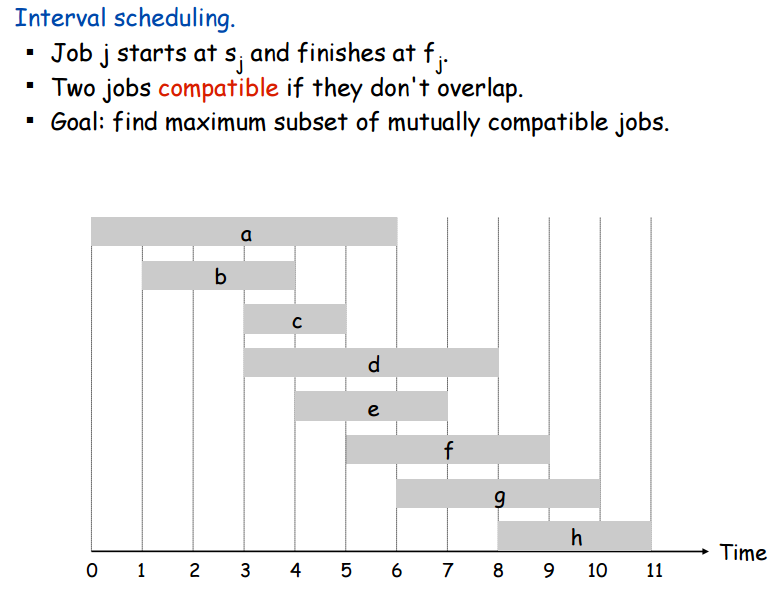
\includegraphics[width=0.65\linewidth]{figures/scheduling.png}
    \caption{Interval Scheduling}
    \label{fig:my_label}
\end{figure}
\noindent
\textbf{Interval Scheduling Algorithm}:
\begin{algorithm}[H]
\caption{Interval Scheduling Algorithm}
\begin{algorithmic}[1]
\Procedure{IntervalScheduling}{$[s_1,f_1],[s_2,f_2],\dots,[s_n,f_n]$}
\State $R$ is the set of requests
\State $A \gets \emptyset$
\While{$R \neq \emptyset$}
\State select a request $i$ in $R$ with the smallest finishing time
\State add $i$ to $A$
\State remove all requests from $R$ that are incompatible with $i$
\EndWhile
\State \Return $A$
\EndProcedure
\end{algorithmic}
\end{algorithm}
\noindent
\textbf{Running time of Interval Scheduling Algorithm}: $O(n\log n)$\\
\textbf{Correctness of Interval Scheduling Algorithm}:
Since the algorithm always selects the request with the smallest finishing time, it is clear that the algorithm will always select a compatible request.\\
\textbf{Arguing optimality}:\\


\section{Minimum Spanning Trees}
Consider a connected graph $G=(V,E)$, such that each edge $e=(v,w)$ of $E$, there is an associated cost $c_e$.\\
\textbf{Goal}: Find a spanning tree $T$ of $E$ so that the graph $G'=(V,T)$ has minimum cost.\\
\textbf{Example}:\\
\begin{center}
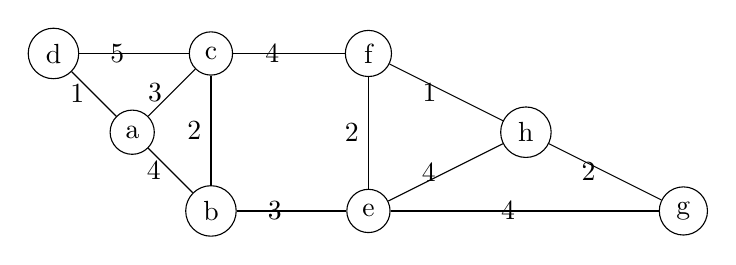
\begin{tikzpicture}
\centering
\node[shape=circle,draw=black] (A) at (1,1) {a};
\node[shape=circle,draw=black] (B) at (2,0) {b};
\node[shape=circle,draw=black] (C) at (2,2) {c};
\node[shape=circle,draw=black] (D) at (0,2) {d};
\node[shape=circle,draw=black] (E) at (4,0) {e};
\node[shape=circle,draw=black] (F) at (4,2) {f};
\node[shape=circle,draw=black] (G) at (8,0) {g};
\node[shape=circle,draw=black] (H) at (6,1) {h};
\path [-] (A) edge node[left] {4} (B);
\path [-] (A) edge node[left] {3} (C);
\path [-] (A) edge node[left] {1} (D);
\path [-] (B) edge node[left] {2} (C);
\path [-] (B) edge node[left] {3} (E);
\path [-] (C) edge node[left] {5} (D);
\path [-] (C) edge node[left] {4} (F);
\path [-] (E) edge node[left] {4} (G);
\path [-] (E) edge node[left] {2} (F);
\path [-] (F) edge node[left] {1} (H);
\path [-] (G) edge node[left] {2} (H);
\path [-] (E) edge node[left] {4} (H);
\end{tikzpicture}\\
\end{center}

\textbf{Greedy approach 1}:\\
\begin{itemize}
    \item Start with an empty set of edges $T$.
    \item Repeat until $T$ forms a spanning tree:
    \begin{itemize}
        \item Select an edge $e$ of minimum cost.
        \item If $T \cup \{e\}$ does not contain a cycle, then add $e$ to $T$.
    \end{itemize}
\end{itemize}
\textbf{krukals algorithm}:
\begin{algorithm}[H]
\caption{Krukals algorithm}
\begin{algorithmic}[1]
\Procedure{Krukals}{$G$}
\State $T \gets \emptyset$
\While{$T$ is not a spanning tree}
\State select an edge $e$ of minimum cost
\If{$T \cup \{e\}$ does not contain a cycle}
\State add $e$ to $T$
\EndIf
\EndWhile
\State \Return $T$
\EndProcedure
\end{algorithmic}
\end{algorithm}

\noindent
\textbf{Running time of Krukals algorithm}: $O(m\log n)$\\
\textbf{Greedy approach 2}:
\begin{itemize}
    \item Start with an empty set of edges $T$.
    \item Start with a node $s$.
    \begin{itemize}
        \item Add an edge $e=(s,v)$ of minimum cost to $T$.
    \end{itemize}
    \item Repeat until $T$ forms a spanning tree:
\end{itemize}
\textbf{Prims algorithm}:
\begin{algorithm}[H]
\caption{Prims algorithm}
\begin{algorithmic}[1]
\Procedure{Prims}{$G$}
\State $T \gets \emptyset$
\State $s \gets$ an arbitrary node
\While{$T$ is not a spanning tree}
\State add an edge $e=(s,v)$ of minimum cost to $T$
\State $s \gets v$
\EndWhile
\State \Return $T$
\EndProcedure
\end{algorithmic}
\end{algorithm}
\noindent
\textbf{Running time of Prims algorithm}: $O(m\log n)$\\
\textbf{minimum spanning tree of example graph}:\\
the minimum spanning tree sequence is $d,a,c,b,e,f,h,g$.\\
\noindent

\textbf{Greedy approach 3}:\\
\begin{itemize}
    \item Start with the full graph $G=(V,E)$.
    \item Delete an edge from $G$
    \begin{itemize}
        \item the edge of maximum cost
    \end{itemize}
    \item Repeat until $G$ forms a spanning tree:
\end{itemize}
\textbf{Reverse-delete algorithm}:
\begin{algorithm}[H]
\caption{Reverse-delete algorithm}
\begin{algorithmic}[1]
\Procedure{ReverseDelete}{$G$}
\State $T \gets G$
\While{$T$ is not a spanning tree}
\State delete an edge $e$ of maximum cost from $T$
\EndWhile
\State \Return $T$
\EndProcedure
\end{algorithmic}
\end{algorithm}
\noindent
For when two edges have the same cost, use distinct labels to distinguish them.\\

\noindent
\textbf{Optimal with Priorty Queue}:\\
Add PQ to Prim's algorithm.\\
\begin{algorithm}[H]
\caption{Optimal with Priorty Queue}
\begin{algorithmic}[1]
\Procedure{Optimal}{$G$}
\State $T \gets \emptyset$
\State $s \gets$ an arbitrary node
\State $PQ \gets$ empty priority queue
\For{each node $v$}
\State add $v$ to $PQ$ with key $\infty$
\EndFor
\State decrease key of $s$ to 0
\While{$PQ$ is not empty}
\State $v \gets$ node with minimum key in $PQ$
\State add an edge $e=(s,v)$ of minimum cost to $T$
\State $s \gets v$
\For{each edge $e=(v,w)$ incident to $v$}
\If{$w$ is in $PQ$}
\State decrease key of $w$ to $c_e$
\EndIf
\EndFor
\EndWhile
\State \Return $T$
\EndProcedure
\end{algorithmic}
\end{algorithm}
\noindent
\textbf{Running time of Optimal with Priorty Queue}: $O(m\log n)$\\

\section{Clustering}
\begin{itemize}
    \item a collection of $n$ objects
    \item they have different degrees of similarity
    \item we want to organise them into coherent groups
    \item there is a notion of distance between objects
\end{itemize}
\noindent
\textbf{Definition}:
\begin{itemize}
    \item Given a set $U$ of $n$ elements, a $k-$clustering of $U$ is a partition of $U$ into non-empty subsets $C_1,C_2,\dots,C_k$.
    \item The spacing of a $k-$clustering is the minimum distance between any pair of points in different clusters.
\end{itemize}
\textbf{Goal}:Among all possible $k-$clusterings, find one with minimum spacing.\\
\textbf{Example}:\\
\begin{center}
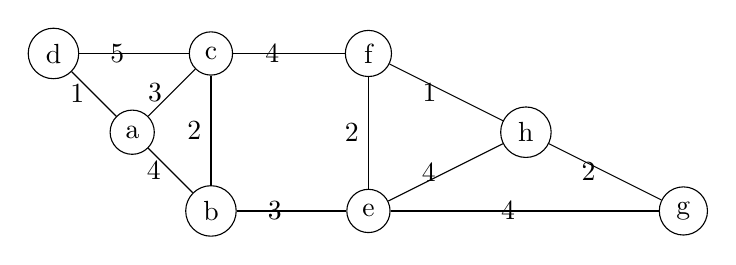
\begin{tikzpicture}
\centering
\node[shape=circle,draw=black] (A) at (1,1) {a};
\node[shape=circle,draw=black] (B) at (2,0) {b};
\node[shape=circle,draw=black] (C) at (2,2) {c};
\node[shape=circle,draw=black] (D) at (0,2) {d};
\node[shape=circle,draw=black] (E) at (4,0) {e};
\node[shape=circle,draw=black] (F) at (4,2) {f};
\node[shape=circle,draw=black] (G) at (8,0) {g};
\node[shape=circle,draw=black] (H) at (6,1) {h};
\path [-] (A) edge node[left] {4} (B);
\path [-] (A) edge node[left] {3} (C);
\path [-] (A) edge node[left] {1} (D);
\path [-] (B) edge node[left] {2} (C);
\path [-] (B) edge node[left] {3} (E);
\path [-] (C) edge node[left] {5} (D);
\path [-] (C) edge node[left] {4} (F);
\path [-] (E) edge node[left] {4} (G);
\path [-] (E) edge node[left] {2} (F);
\path [-] (F) edge node[left] {1} (H);
\path [-] (G) edge node[left] {2} (H);
\path [-] (E) edge node[left] {4} (H);
\end{tikzpicture}\\
\end{center}
\textbf{Greedy approach}:\\
\begin{itemize}
    \item Pick two objects $p_i$ and $p_j$ with minimum distance $d(p_i,p_j)$.
    \item Connect them with an edge $e=(p_i,p_j)$.
    \item Continue like this until we have $k$ clusters.
    \item If the edge $e$ under consideration connects two object $p_i$ and $p_j$ already in the same cluster, then discard $e$.
\end{itemize}
\textbf{kruskals algorithm}:
\begin{algorithm}[H]
\caption{kruskals algorithm for clustering}
\begin{algorithmic}[1]
    \Require A graph $G = (V,E)$
    \Ensure A minimum spanning tree of $G$ with $k$ clusters
    
    \Procedure{Kruskal}{$G,k$}
      \State $T \gets \emptyset$
      \State $C \gets \{ \{v\} \mid v \in V \}$ \Comment{Initial clusters}
      \State Sort edges in $E$ in increasing order of weight
      \For{$\{u,v\} \in E$}
        \If{$C$ contains $k$ clusters}
          \State \textbf{break}
        \EndIf
        \If{clusters containing $u$ and $v$ are different in $C$}
          \State $T \gets T \cup \{\{u,v\}\}$
          \State merge clusters containing $u$ and $v$ in $C$
        \EndIf
      \EndFor
      \State \textbf{return} $T$
    \EndProcedure
\end{algorithmic}
\end{algorithm}
\noindent
For Given example, the result of divide them into 3 clusters is:\\
\begin{equation*}
    \{a,b,c,d\},\{e,f,h\},\{g\}
\end{equation*}
\noindent





















\end{document}